%-------------------------------------------------------------------------------
%                            BAB III
%               		METODOLOGI PENELITIAN
%-------------------------------------------------------------------------------

\chapter{METODOLOGI PENELITIAN}

\section{Tempat dan Waktu Penelitian}
\setlength\parindent{30pt} Penelitian ini dilakukan di Jurusan Informatika, Fakultas Matematika dan Ilmu Pengetahuan Alam, Universitas Syiah Kuala Banda Aceh. Waktu yang diperlukan untuk melakukan penelitian ini kurang lebih selama lima bulan, yang dimulai dari bulan Juni 2018 sampai bulan Desember 2018.

% Please remember to add \use{multirow} to your document preamble in order to suppor multirow cells
\begin{table}[H]
	\center
	\caption{Jadwal Penelitian.}
	\label{jadwal}
	\begin{tabular}{|c|l|l|l|l|l|l|l|}
		\hline
		\multirow{2}{*}{No} & \multirow{2}{*}{Keterangan} 	& \multicolumn{6}{c|}{Bulan}           																										\\ \cline{3-8} 
							&                           	& Jul				& Agt  			& Sep			& Okt			& Nov			& Des 					\\ \hline       
		1                   & Studi literatur           	&\cellcolor{gray}	&\cellcolor{gray}	&                   &                   &                   &                       	\\ \hline
		2                   & Penulisan Proposal           	&                   &\cellcolor{gray}	&\cellcolor{gray}	&                   &                   &                        	\\ \hline
		3                   & Pengembangan Aplikasi         &                   &                   & \cellcolor{gray}  & \cellcolor{gray} 	& \cellcolor{gray}  &                            \\ \hline
		4                   & Evaluasi Sistem               &                   &                   &           		&             		&\cellcolor{gray}	&  \cellcolor{gray}    \\ \hline
		5                   & Penulisan Laporan Akhir       &                   &                   &                   &        			&      				& \cellcolor{gray}     \\ \hline
	\end{tabular}
\end{table}

\section{Alat dan Bahan}
Alat yang digunakan pada penelitian ini adalah sebagai berikut :

\begin{enumerate}[a.]
\item Perangkat Keras (\textit{Hardware})
	\begin{itemize}
		\item 1 unit Laptop ASUS ROG Intel(R) Core(TM) i7 6700HQ
		\item RAM 8 GB DDR3
		\item Harddisk 1 TB
		\item 1 unit Android Samsung S7
	\end{itemize}

\item Perangkat Lunak (\textit{Software})
	\begin{itemize}
		\item Visual Studio Code
		\item Cordova 7.0.0
		\item Ionic Framework 3
		\item SDK Android 27.0.1
	\end{itemize}
\end{enumerate}

\section{Metode Penelitian}
Skema dari alur tahapan penelitian dapat dilihat pada Gambar \ref{alur}
\vspace{-0.4cm}
\begin{figure}[H]
	\center
	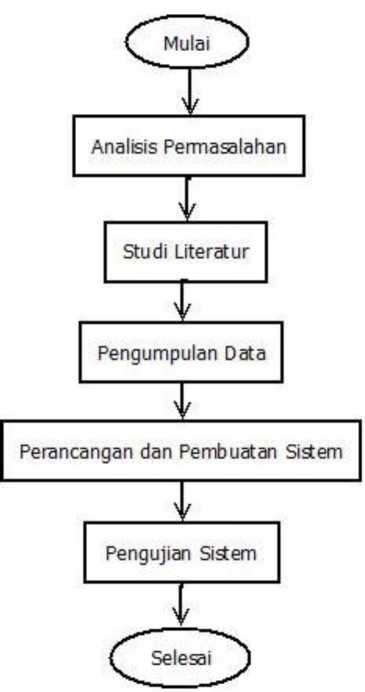
\includegraphics [width = 6cm, height= 10cm]{gambar/alur2}
	\caption{Diagram Alir Penelitian}
	\label{alur}
\end{figure}

\subsection{Analisis Permasalahan}
Aplikasi ini merupakan aplikasi berbasis mobile yang berguna untuk membantu pangkalan gas LPG Subsidi 3 Kg dalam melakukan pelaporan penyaluran tabung gas subsidi. Aplikasi ini juga membantu agen gas LPG selaku distributor dan pengawasan dari pangkalan gas untuk melakukan rekap laporan penyaluran tabung gas 3 Kg. Aplikasi ini melakukan pelaporan penyaluran tabung gas subsidi dengan menggunakan NIK(Nomor Induk Kependudukan) dan no telepon sebagai data acuan yang valid. Setelah itu data tersebut langsung di kirim langsung ke agen gas LPG bersangkutan. Adapun fitur-fitur yang terdapat pada aplikasi ini adalah sebagai berikut
\begin{itemize}
		\itemsep0em
		\item Masuk ke dalam aplikasi.
		\item Melihat jadwal pasokan tabung.
		\item Mencatat penjualan tabung gas menggunakan NIK sebagai acuan.
		\item Mencetak kartu kendali untuk konsumen.
		\item Mengubah profile biodata user.
\end{itemize}

\subsection{Studi Literatur}
Studi literatur dilakukan dengan mencari jurnal baik nasional maupun internasional, buku, serta beberapa literatur elektronik yang diunduh dari internet yang terkait dengan penelitian ini. Studi literatur juga diperoleh dengan meneliti aplikasi atau perangkat lunak yang berkaitan dengan penelitian. Studi literatur digunakan sebagai bahan referensi selama proses penelitian.

\subsection{Pengumpulan Data}
Data yang digunakan dalam penelitian ini adalah data penyaluran tabung ke masyarakat dan format pelaporan yang dipakai oleh pangkalan. Data tersebut didapatkan dari agen dan pangkalan yang menjadi objek penelitian.

\subsection{Perancangan dan Pembuatan Sistem}
Dalam merancang aplikasi ini, digunakan metode pengembangan perangkat lunak yaitu Scrum. Metode Scrum sangat fleksibel terhadap perubahan-perubahan sehingga cocok digunakan pada aplikasi ini. Berikut merupakan tahapan perancangan sistem yang akan dilakukan:

\begin{enumerate}[1.]
	\item \emph {Planning}
	
	Pada tahap ini dilakukan analisa terhadap masalah yang terjadi di lapangan dalam penelitian ini yaitu pangkalan gas LPG 3 Kg dan mencari solusi yang akan memecahkan masalah tersebut dengan mengembangkan suatu sistem. Setelah itu dilakukan tahap inisiasi awal pengembangan sistem yaitu melakukan analisis kebutuhan pada setiap pengguna sistem yaitu Agen dan Pangkalan Gas LPG yang dilanjutkan dengan membuat \textit{storyboard} yaitu gambaran yang menceritakan jalannya sistem yang dibuat secara singkat.
	
	

	\item \textit{Design}
	
	\par Tahap ini fokus pada desain pembuatan perangkat lunak termasuk struktur data, arsitektur perangkat lunak, representasi antarmuka dan prosedur pengkodean. Proses tahap ini dilakukan dengan terlebih dahulu mengidentifikasi persona, \textit{value proposition canvas} (vpc), membuat use case diagram yang ditunjukkan pada Gambar \ref{usecase} untuk setiap aktor dan storyboard. Proses tersebut dilakukan untuk memastikan setiap desain dan cara kerja aplikasi yang dibangun dapat digunakan oleh masing-masing kelompok pengguna.
	\newpage
	\par Perancangan sistem terbagi 2 yaitu aplikasi \textit{mobile web} yang akan digunakan oleh Pangkalan Gas LPG untuk melakukan pencatatan penyaluran tabung gas dan \textit{web admin} yang akan digunakan oleh Agen Gas LPG untuk melakukan rekapitulasi data penyaluran. Adapun beberapa contoh desain tampilan antarmuka dari aplikasi yang akan dirancang seperti Gambar \ref{appPangkalan} dan Gambar \ref{appAgen}.
	
	\vspace{-0.4cm}
	\begin{figure}[H]
		\center
		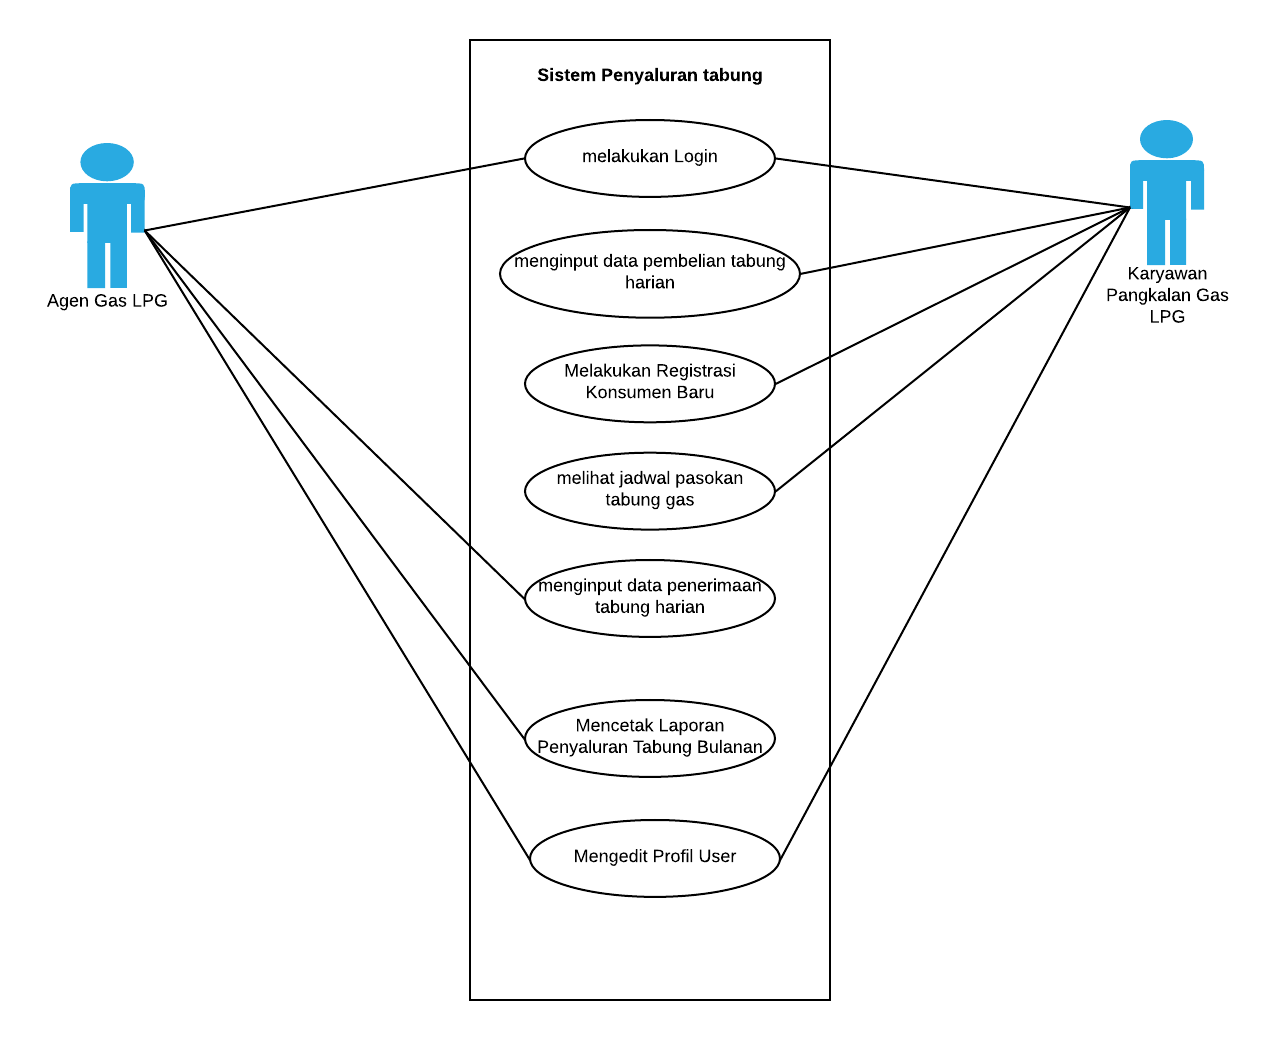
\includegraphics [width = 12cm, height= 11cm]{gambar/use-case}
		\caption{Diagram Use-Case}
		\label{usecase}
	\end{figure}
	
	
	\begin{figure}[H]
		\center
		\begin{subfigure}[t]{6cm}
			\center
		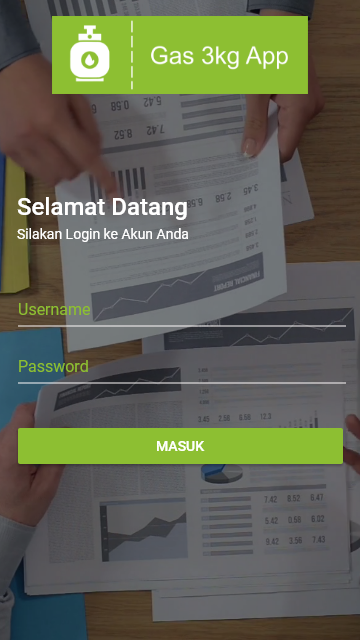
\includegraphics [width = 6cm]{gambar/and/login}
		\caption{Halaman Login}\label{login}		
		\end{subfigure}\hspace{0.3cm}
		\begin{subfigure}[t]{6cm}
			\center
			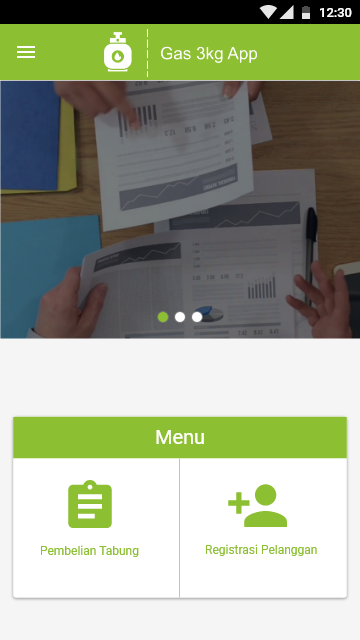
\includegraphics [width = 6cm]{gambar/and/beranda}
			\caption{Menu Utama}\label{beranda}		
		\end{subfigure}\vspace{0.3cm}
		\begin{subfigure}[t]{6cm}
			\center
			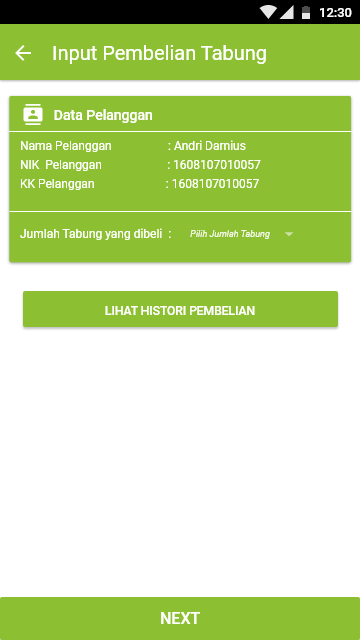
\includegraphics [width = 6cm]{gambar/and/pembelian}
			\caption{Halaman Pembelian Tabung}\label{pembelian}		
		\end{subfigure}\hspace{0.3cm}
		\begin{subfigure}[t]{6cm}
			\center
			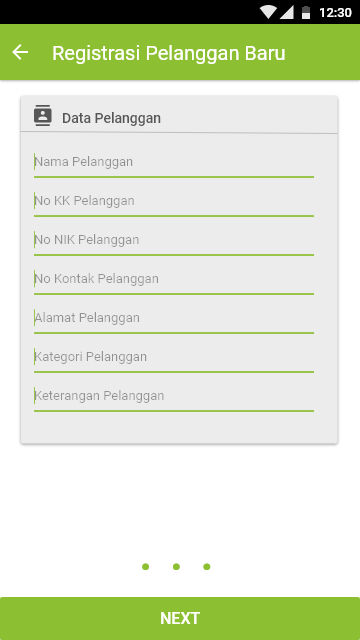
\includegraphics [width = 6cm]{gambar/and/registrasi}
			\caption{Halaman Registrasi}\label{registrasi}		
		\end{subfigure}
		\caption{Tampilan aplikasi untuk pangkalan gas LPG }\label{appPangkalan}
	\end{figure}

	\begin{figure}[H]
		\center
		\begin{subfigure}[t]{7cm}
			\center
			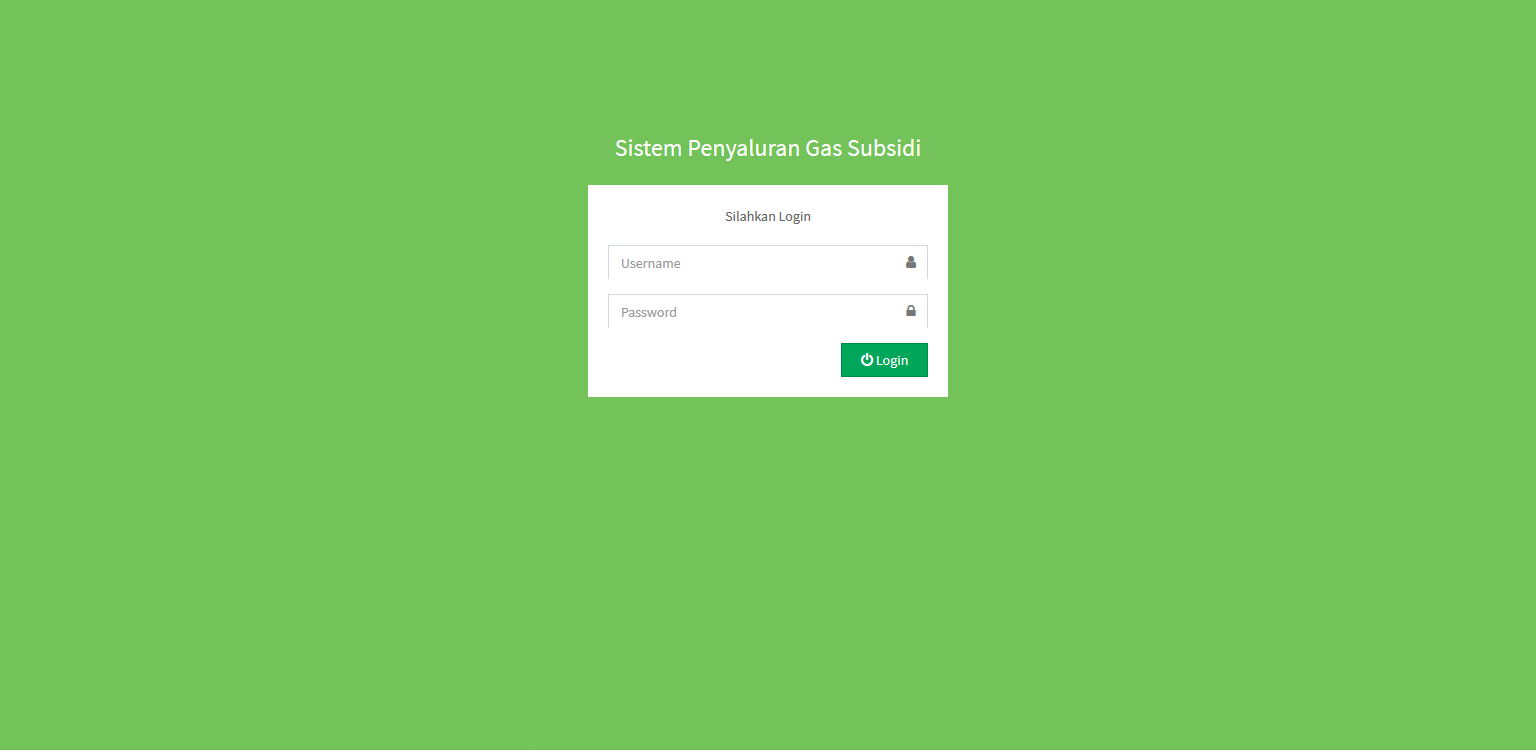
\includegraphics [width = 7cm]{gambar/web/login}
			\caption{Halaman Login}\label{login}		
		\end{subfigure}\hspace{0.2cm}
		\begin{subfigure}[t]{7cm}
			\center
			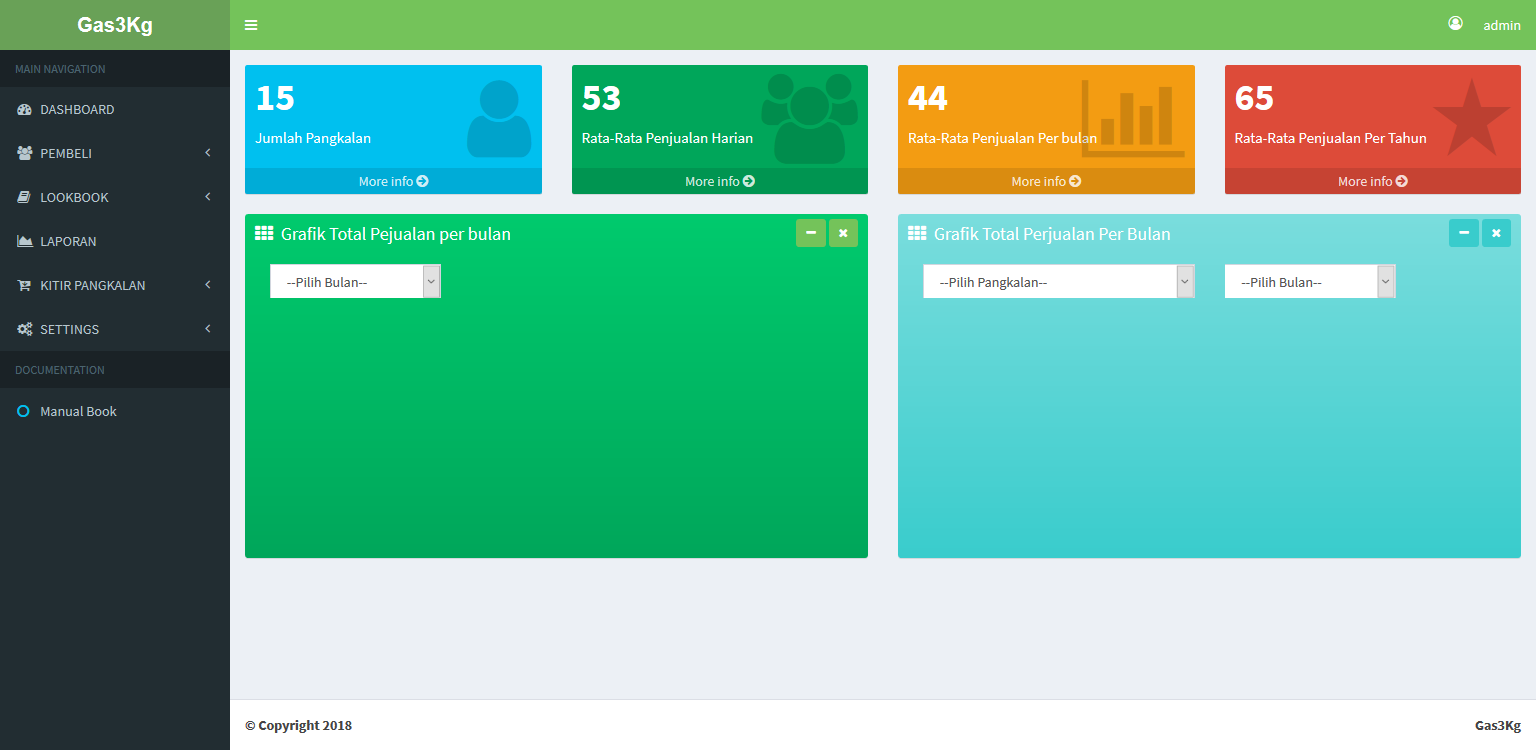
\includegraphics [width = 7cm]{gambar/web/dashboard}
			\caption{Menu Utama}\label{beranda}		
		\end{subfigure}
		\caption{Tampilan aplikasi untuk agen gas LPG }\label{appAgen}
	\end{figure}

	
	\item \textit{Coding}
	
	Pada tahapan ini, dilakukan implementasi terhadap desain yang telah dibuat sebelumnya ke dalam bentuk program. Penulisan kode program dalam penelitian ini menggunakan Ionic Framework yang ditulis dalam bahasa pemrograman Typescript untuk aplikasi berbasis Android dan untuk web service yang akan digunakan oleh aplikasi untuk berkomunikasi dengan database akan menggunakan Google App Engine yang ditulis dalam bahasa pemrograman Java.

	 \item \textit{Testing}
	
	Tahapan \textit{testing} yang dilakukan diantaranya adalah sebagai berikut:
	\begin{enumerate}[a.]
			\itemsep0em
			\item \textit{Usability}
			\newline Pengujian \textit{usability} digunakan untuk mengetahui seberapa mudah aplikasi dapat dijalankan oleh pengguna. Teknik pengujian \textit{usability} yang digunakan adalah dengan memberikan kuesioner kepada setiap kelompok user yaitu agen gas LPG dan pangkalan gas LPG. Jenis pertanyaan yang ada pada kuesioner mengacu pada kuesioner SUS (\textit{System Usability Scale}). Dalam pengujian \textit{usability} ini, melibatkan sekitar 8 pengguna yang berbeda.
			\item \textit{Unit Testing}
			\newline Unit testing fokus pada verifikasi pada unit yang terkecil pada desain perangkat lunak (komponen atau modul perangkat lunak). Karena dalam sebuah perangkat lunak banyak memiliki unit-unit kecil maka untuk mengujinya biasanya dibuat program kecil atau main program) untuk menguji unit-unit perangkat lunak.
		
	\end{enumerate}
	
	
\end{enumerate}


% Baris ini digunakan untuk membantu dalam melakukan sitasi
% Karena diapit dengan comment, maka baris ini akan diabaikan
% oleh compiler LaTeX.
\begin{comment}
\bibliography{daftar-pustaka}
\end{comment}
